\documentclass{beamer}

%\usetheme{Darmstadt}
%\usefonttheme[onlylarge]{structurebold}
%\setbeamerfont*{frametitle}{size=\normalsize,series=\bfseries}
%\setbeamertemplate{navigation symbols}{}
\usepackage{listings}

% Standard packages
% Author, Title, etc.

\title
{%
  Exaile Media Player:\\
  An Open Source Introspection....?? %
}

\author
{
  Abhishek Mukherjee \and
  Roy Wellington
}

% The main document

\begin{document}
\lstset{language=Python}

\begin{frame}
  \titlepage
\end{frame}

\begin{frame}{Outline}
  \tableofcontents
\end{frame}


\section{Introduction}

\subsection{Exaile}

\begin{frame}{Wotsit do?}
  \begin{quote}
    Exaile is a music manager and player for GTK+ written in Python.
  \end{quote}
  \begin{figure}
    %FIXME: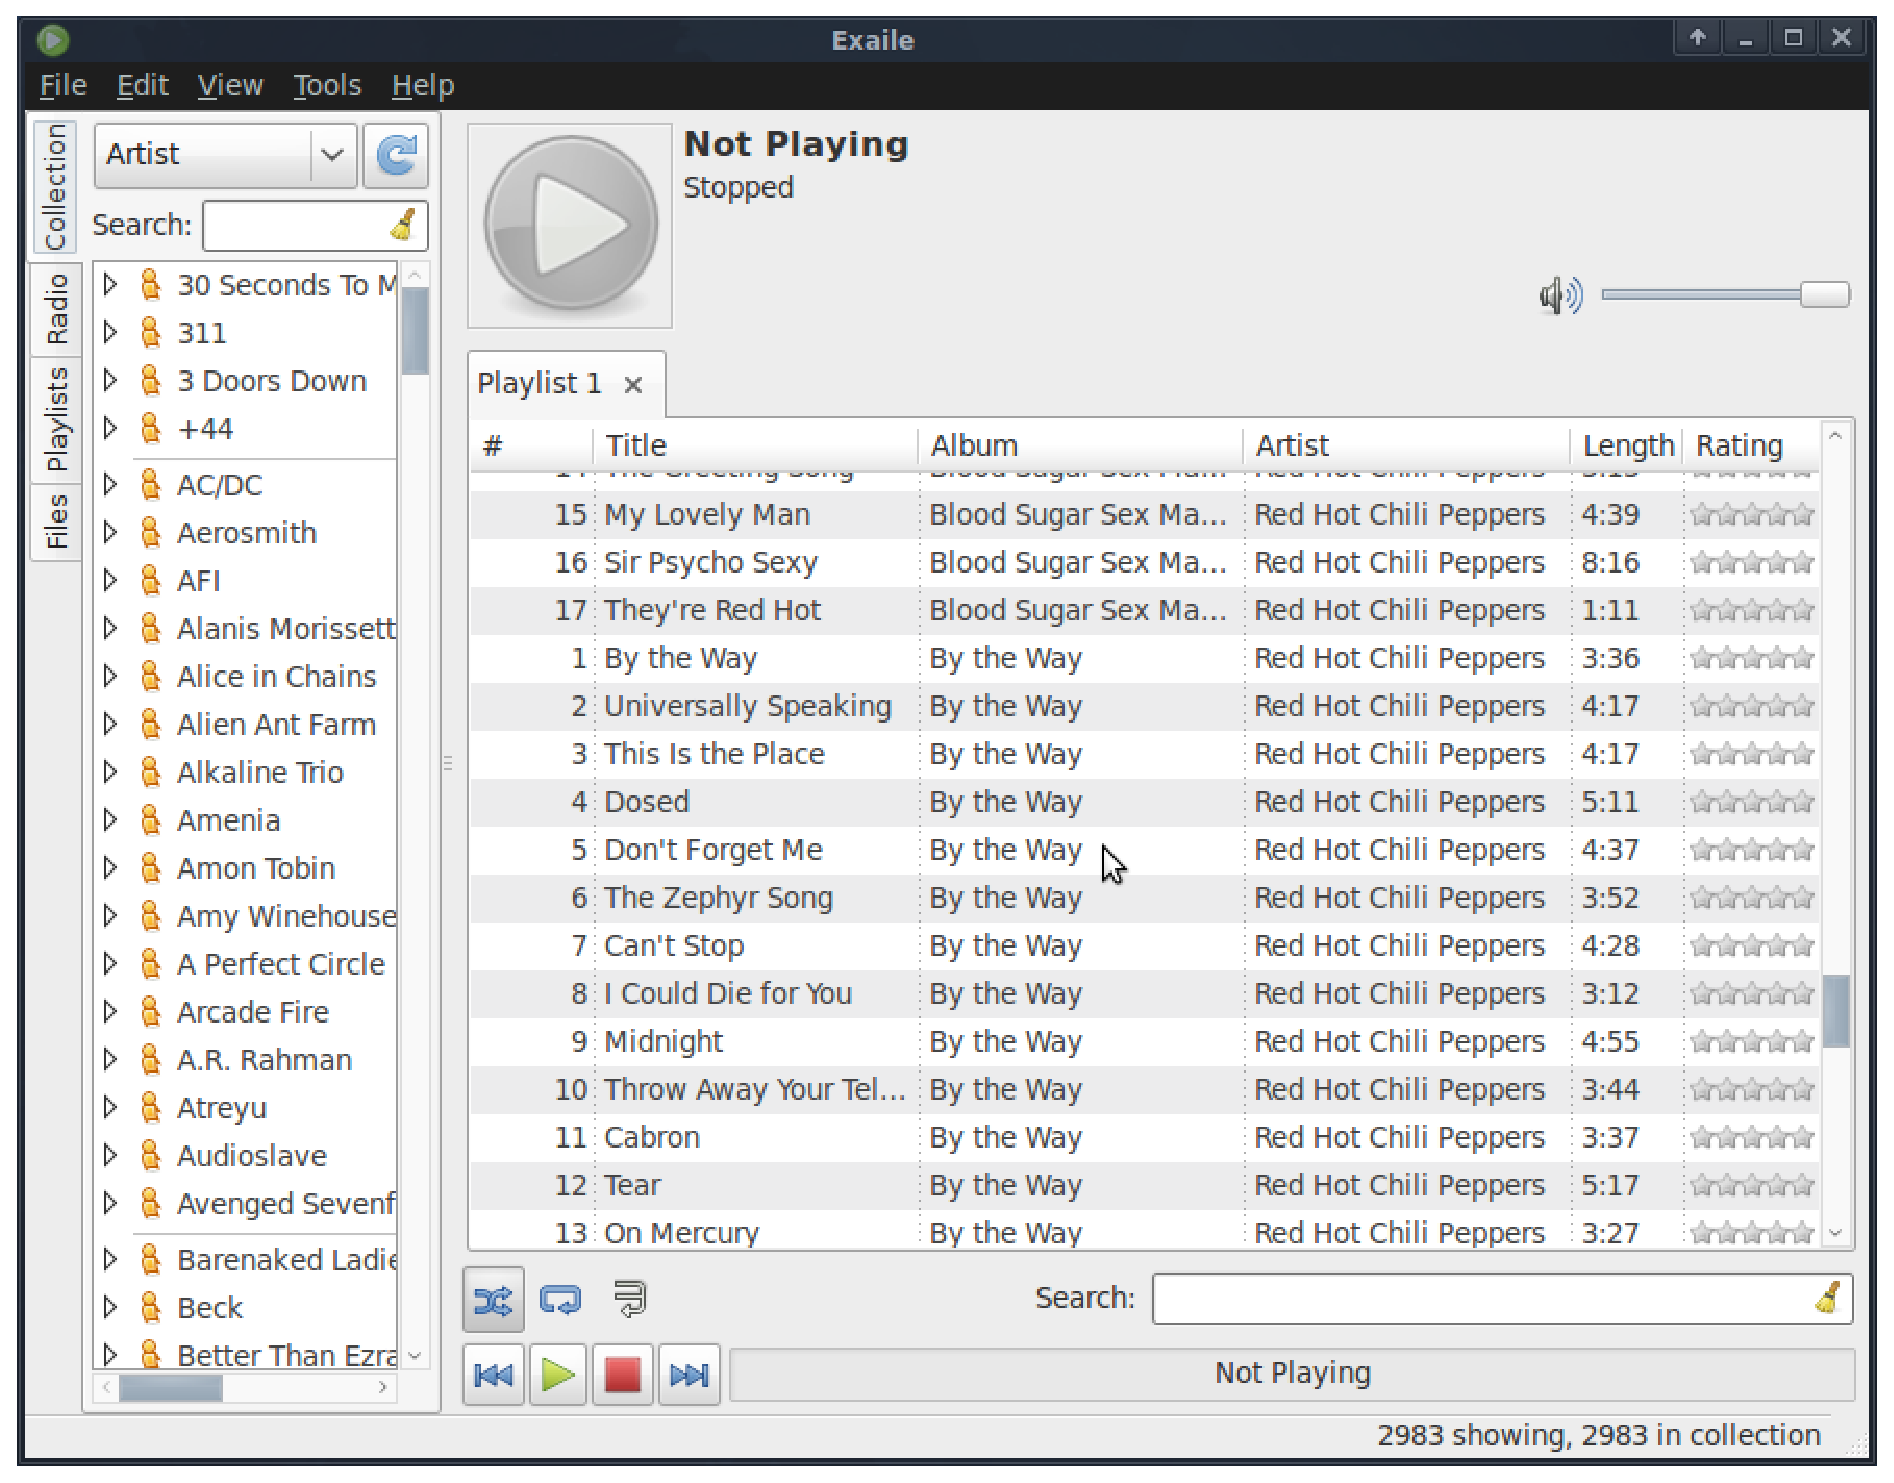
\includegraphics[height=60mm]{images/exaile.eps}
    \caption{The Program}
  \end{figure}
\end{frame}

\begin{frame}{Project Statistics}
  Code statistics for Exaile (as of -r2699)
  \begin{itemize}
    \item 24079 lines of Python
    \item $\sim$5000 lines of XML
    \item $\sim$166.5k lines of translations
    \item 724 lines of test (that don't work)
	\item Plugin code:
	\begin{itemize}
      \item 21916 lines of Python (plugins)
      \item 4286 lines of XML (plugins)
      \item 2329 lines of C (plugins)
      \item 581 lines of tests (plugins)
	\end{itemize}
  \end{itemize}
\end{frame}

\section{Features}

\subsection{Selection Randomization}

\begin{frame}{Feature: Selection randomization}
  \begin{itemize}
     \item Exaile originally only allows randomization of an entire playlist
     \item Our change allows a user to randomize a selected part of a playlist.
  \end{itemize}
\end{frame}

\begin{frame}{Why randomize?}
  Many people ask why not just use shuffle.
  \begin{itemize}
    \item Shuffle doesn't allow you to see what's next/previous.
	\item Shuffle doesn't allow you to custom order a subset of the playlist.
  \end{itemize}
\end{frame}

\subsubsection{The Old Way}
\begin{frame}{The Old Way}
  \begin{itemize}
    \item Select this from the menu:

    %FIXME:
\includegraphics[keepaspectratio]{images/tools-menu}
    \item And the entire playlist is randomized.
	\item What if we only want to randomize a subset of the playlist?
  \end{itemize}
\end{frame}

\subsubsection{The New Way}
\begin{frame}{The New Way}
  \begin{itemize}
  \item Select several things in your playlist:
  \item Right click, then use this menu-item:

    %FIXME: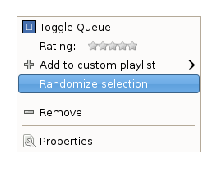
\includegraphics[keepaspectratio]{images/randomize-menu-item}
  \item The selected items are randomized.
  \end{itemize}
\end{frame}

\subsection{Unified Engine}

\begin{frame}{Feature: Unified engine}
  \begin{itemize}
    \item Exaile has two engines: "Normal" and "Unified"
	\item The normal engine is boring.
	\item The unified engine is shiny.
  \end{itemize}
\end{frame}

\subsubsection{The Old Way}
\begin{frame}{The Old Way}
  \begin{itemize}
    \item The normal engine just plays one song at a time.
	\item The unified engine allows us to:
	  \begin{itemize}
	    \item Crossfade
		\item Gapless playback
		\item \textit{(insert other potentially shiny here)}
      \end{itemize}
	\item It doesn't work. Playback randomly skips, buggy.
  \end{itemize}
\end{frame}

\subsubsection{The\ldots\ not New Way}
\begin{frame}{The\ldots\ not New Way}
  \begin{itemize}
    \item Fix/rewrite of the unified engine didn't happen.
	\item Engine turned out to be complex:
	\item \textgreater 1500 lines of code. (And not simple GUI stuff.)
  \end{itemize}
\end{frame}


\subsection{Awn Integration}
\begin{frame}{Feature: Awn Integration}
Exaile used to have a plugin (before the massive rewrite in 0.3) to interface
with awn properly. This no longer worked and had to be rewritten for the new
architecture
\end{frame}

\begin{frame}{What's Awn}
  \begin{itemize}
    \item Awn is a COMPLETELY original task bar/manager
    \item Also has notification area and is very extensible
  \end{itemize}
  \begin{figure}
    \centering
    %FIXME:
\includegraphics[width=100mm]{images/awn}
    \caption{Completely original task bar}
  \end{figure}
\end{frame}

\subsubsection{The Old Way}
\begin{frame}{The Old Way}
  \begin{figure}
    \centering
    %FIXME:
\includegraphics[width=100mm]{images/awn}
    \caption{Same example of completely original task bar}
  \end{figure}
\end{frame}

\subsubsection{The New Way}
\begin{frame}{The New Way}
  \begin{figure}
    \centering
    %FIXME: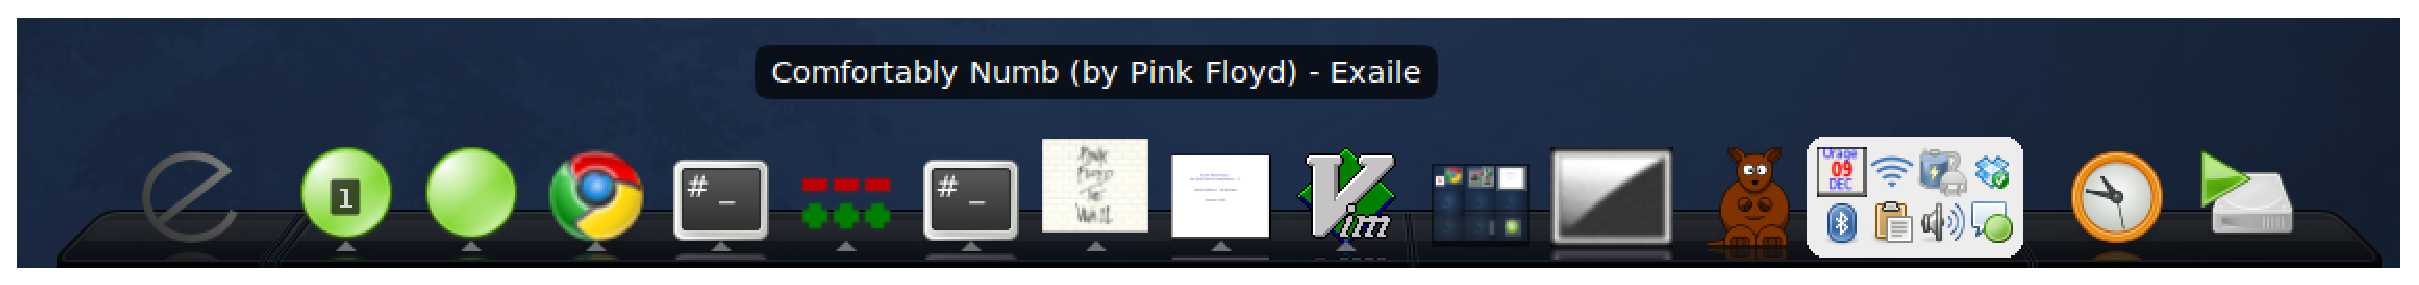
\includegraphics[width=100mm]{images/awn-new}
    \caption{New and improved task bar}
  \end{figure}
\end{frame}

\subsection{Planned features}
\begin{frame}{Planned feature}
  \begin{itemize}
    \item There were a few features that we were not able to implement but
      were in the process of discussing and coding
    \item Those features were:
    \begin{itemize}
      \item Stabilize Unified Playback engine
      \item Reduce memory footprint
      \item Fix tests (G's wanted to do this for a while, but there's a
        \emph{lot} wrong with them)
      \item Kill all \lstinline!except:!'s (Considered bad form in python)
      \item Migrate current installation system (GNU Makefiles) to
        Distribute\footnote{Spiritual successor for setuptools, an advanced
        package management tool for Python. Not maintained by a ``lunatic''}
    \end{itemize}
  \end{itemize}
  All of these features have been discussed with the lead devs and approved.
  The work for them just has to be done.
\end{frame}

\section{Community Integration}
\begin{frame}{G's experience}
  \begin{itemize}
    \item Pretty easy
    \begin{enumerate}
      \item Decided I was going to write a plugin for Exaile (MPRIS plugin)
      \item Wrote the plugin
      \item Talked with reacocard (one of the three creators) about it.
      \item Got more acquainted with the people in the room, began picking
        up bugs in the bug tracker
    \end{enumerate}
    \item At this point it's more along the lines of:
\begin{verse}
  $<$G$>$ reacocard, I'm implementing feature X

  $<$reacocard$>$ G, Yea, we've needed that
\end{verse}
  \end{itemize}
\end{frame}

\begin{frame}{Roy's experience}
\begin{quote}
Roy Wellington: who's reacocard, do you know?

Roy Wellington: I've just been stalking the channel thus far, and I got:

Roy Wellington: 19:33  * reacocard wonders if deathanatos is ever going to say anything :)
\end{quote}
\end{frame}

\begin{frame}{Roy's experience}
  \begin{itemize}
    \item First time I've ever gotten that while stalking in IRC.
	\item Community welcomes those who want to help.
	\item Contact is easy, project seems alive and well.
  \end{itemize}
\end{frame}

\end{document} %
% vim:ts=2 sw=2 et:
